\chapter{Implementacija i korisničko sučelje}
		
		
		\section{Korištene tehnologije i alati}
		
			\textbf{\textit{dio 2. revizije}}
			
			Za komunikaciju u timu korišten je WhatsApp\footnote{\url{https://www.whatsapp.com/}}. Za pisanje koda korišteni su VSCode\footnote{\url{https://code.visualstudio.com/}} i IntelliJ\footnote{\url{https://www.jetbrains.com/idea/}}. Ovi IDE alati su odabrani radi dobre i kvalitetne implementacije i mogučnosti rada u programskim jezicima odabranim za zadatak, te široke dostupnosti dodataka. Za pisanje dokumentacije korišten je TeXstudio\footnote{\url{https://www.texstudio.org/}} Za izradu UML dijagrama korišteni su AstahUML\footnote{\url{https://astah.net/products/astah-uml/}} i IntelliJ.
			Kao udaljeni repozitorij koda, te za upravljanje zajedničkim razvojem koda korišteni su GitHub\footnote{\url{https://github.com/}} i GitLab\footnote{\url{https://gitlab.com/}}.
			Backend aplikacije pisan je u Javi\footnote{\url{https://www.java.com/en/}} koristeći Springboot\footnote{\url{https://spring.io/projects/spring-boot/}}. Frontend je pisan u Reactu\footnote{\url{https://react.dev/}} i JavaScriptu\footnote{\url{https://www.javascript.com/}}. React je popularana biblioteka u JavaScriptu za izradu korisničkih sučelja. Springboot nudi gotove funkcije i resurse koji omogučuju programerima brži i jednostavniji razvoj backenda.
			Baza Podataka realizirana je PostgreSQL\footnote{\url{https://www.postgresql.org/}}. Za hosting backenda, frontenda i baze podataka korišten je besplatan hosting servis Render\footnote{\url{https://render.com/}}.

			\textit{Detaljno navesti sve tehnologije i alate koji su primijenjeni pri izradi dokumentacije i aplikacije. Ukratko ih opisati, te navesti njihovo značenje i mjesto primjene. Za svaki navedeni alat i tehnologiju je potrebno \textbf{navesti internet poveznicu} gdje se mogu preuzeti ili više saznati o njima}.
			
			\eject 
		
	
		\section{Ispitivanje programskog rješenja}
			
			\textbf{\textit{dio 2. revizije}}\\
			
			 \textit{U ovom poglavlju je potrebno opisati provedbu ispitivanja implementiranih funkcionalnosti na razini komponenti i na razini cijelog sustava s prikazom odabranih ispitnih slučajeva. Studenti trebaju ispitati temeljnu funkcionalnost i rubne uvjete.}
	
			
			\subsection{Ispitivanje komponenti}
			\textit{Potrebno je provesti ispitivanje jedinica (engl. unit testing) nad razredima koji implementiraju temeljne funkcionalnosti. Razraditi \textbf{minimalno 6 ispitnih slučajeva} u kojima će se ispitati redovni slučajevi, rubni uvjeti te izazivanje pogreške (engl. exception throwing). Poželjno je stvoriti i ispitni slučaj koji koristi funkcionalnosti koje nisu implementirane. Potrebno je priložiti izvorni kôd svih ispitnih slučajeva te prikaz rezultata izvođenja ispita u razvojnom okruženju (prolaz/pad ispita). }
			
			
			
\subsection{Ispitivanje sustava}

\textbf{Ispitni slučaj 1: Interakcija s sučeljem za prijavu u sustav}

\noindent \textbf{Ulaz:}
\begin{packed_enum}
	\item Otvaranje početne stranice u web pregledniku.
	\item Unos potrebnim podataka za prijavu u sustav (email i lozinka).
	\item Pritisak na akciju "Prijavi se".
\end{packed_enum}

\noindent \textbf{Očekivani rezultat:}
\begin{packed_enum}
	\item Uspješna prijava korisnika u sustav.
	\item Dolazak na naslovnu stranicu sustava.
\end{packed_enum}

\noindent \textbf{Redovni i rubni slučajevi:}
\begin{packed_enum}
	\item Korisnik je unio ispravan email i lozinku.
	\item Korisnik je unio neispravan email ilil lozinku.
	\item Korisnik nije unio email ili lozinku.
	\item Korisnik nije unio ni email ni lozinku.
\end{packed_enum}

\noindent \textbf{Rezultati:}
\begin{packed_enum}
	\item Korisnik je uspješno prijavljen i doveden na naslovnu stranicu.
	\item Korisnik nije prijavljen i javlja se poruka o neispravnom emailu ili lozinki.
	\item Korisnik nije prijavljen te akcija "Prijavi se" nije dostupna.
	\item Korisnik nije prijavljen te akcija "Prijavi se" nije dostupna.
\end{packed_enum}

\begin{figure}[H]
	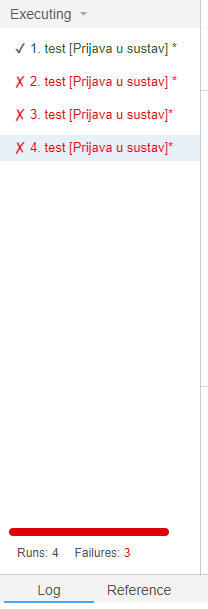
\includegraphics[scale=0.6]{dijagrami/test1.PNG}
	\centering
	\caption{Ispitni slučaj 1. rezultati}
	\label{fig:myChart}
\end{figure}

\begin{figure}[H]
	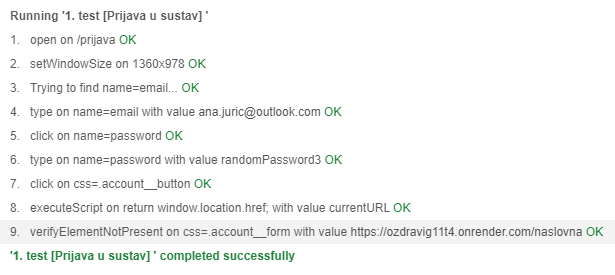
\includegraphics[scale=0.6]{dijagrami/test11.PNG}
	\centering
	\label{fig:myChart}
\end{figure}

\begin{figure}[H]
	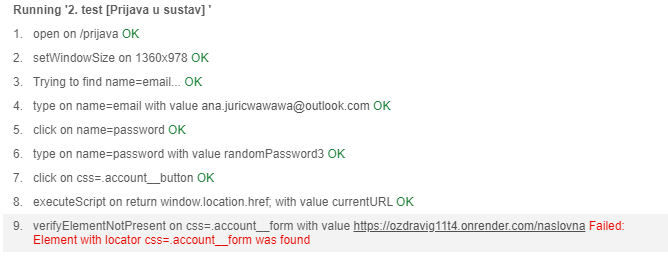
\includegraphics[scale=0.6]{dijagrami/test12.PNG}
	\centering
	\label{fig:myChart}
\end{figure}

\begin{figure}[H]
	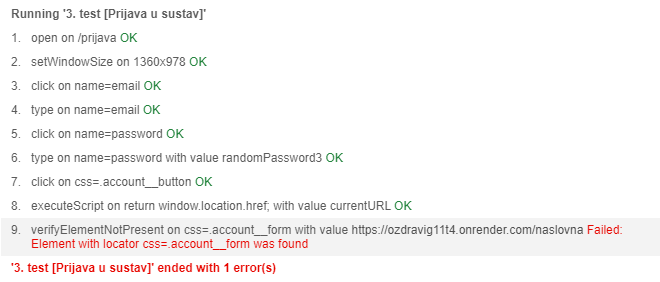
\includegraphics[scale=0.6]{dijagrami/test13.PNG}
	\centering
	\label{fig:myChart}
\end{figure}

\begin{figure}[H]
	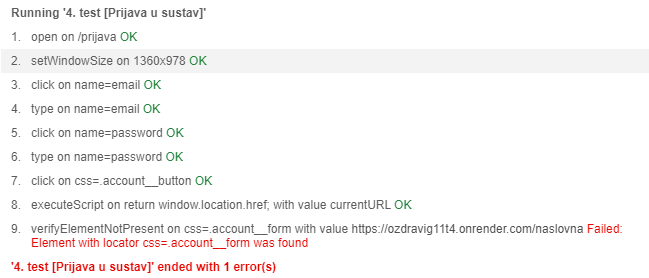
\includegraphics[scale=0.6]{dijagrami/test14.PNG}
	\centering
	\label{fig:myChart}
\end{figure}




\noindent	\textbf{Ispitni slučaj 2: Interakcija s sučeljem za registraciju u sustav}
\\
\noindent \textbf{Ulaz:}
\begin{packed_enum}
	\item Otvaranje početne stranice u web pregledniku.
	\item Unos potrebnim podataka za prijavu u sustav (ime, prezime, email, oib, spol, adresa, lozinka, potvrda lozinke, datum rođenja).
	\item Pritisak na akciju "Registriraj se".
\end{packed_enum}

\noindent \textbf{Očekivani rezultat:}
\begin{packed_enum}
	\item Uspješna registracija korisnika u sustav.
	\item Dolazak na naslovnu stranicu sustava.
\end{packed_enum}

\noindent \textbf{Redovni i rubni slučajevi:}
\begin{packed_enum}
	\item Korisnik je unio ispravne podatke.
	\item Korisnik nije unio sve podatke.
	\item Korisnik je unio neispravni podatak.
	\item Korisnik je unio email ili oib koji već postoji.
\end{packed_enum}

\noindent \textbf{Rezultati:}
\begin{packed_enum}
	\item Korisnik je uspješno registriran i doveden na naslovnu stranicu.
	\item Korisnik nije registriran te akcija "Registriraj se" nije dostupna.
	\item Korisnik nije registriran te akcija "Registriraj se" nije dostupna.
	\item Korisnik nije registriran te se vraća poruka o grešci.
\end{packed_enum}

\begin{figure}[H]
	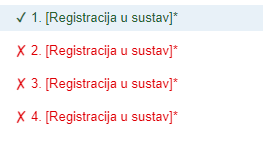
\includegraphics[scale=0.6]{dijagrami/test2.PNG}
	\centering
	\caption{Ispitni slučaj 2. rezultati}
	\label{fig:myChart}
\end{figure}

\begin{figure}[H]
	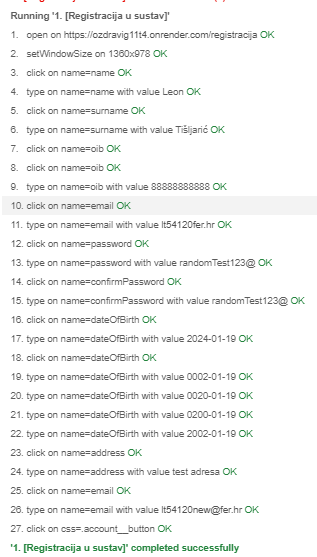
\includegraphics[scale=0.6]{dijagrami/test21.PNG}
	\centering
	\label{fig:myChart}
\end{figure}

\begin{figure}[H]
	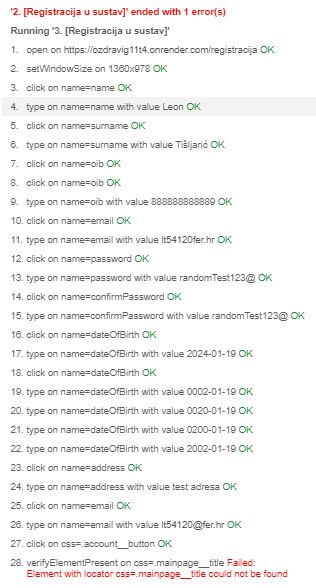
\includegraphics[scale=0.6]{dijagrami/test22.PNG}
	\centering
	\label{fig:myChart}
\end{figure}

\begin{figure}[H]
	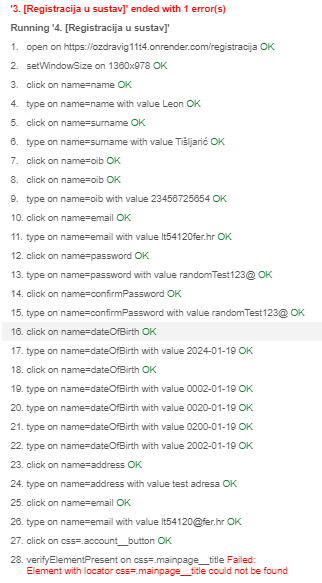
\includegraphics[scale=0.6]{dijagrami/test23.PNG}
	\centering
	\label{fig:myChart}
\end{figure}

\begin{figure}[H]
	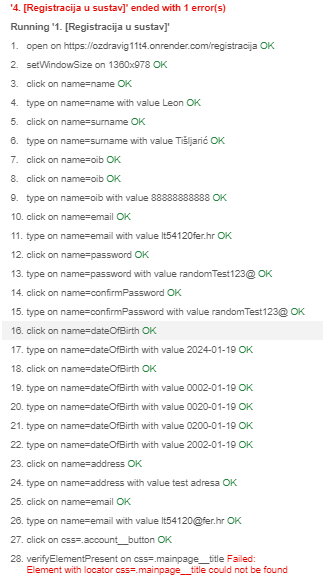
\includegraphics[scale=0.6]{dijagrami/test24.PNG}
	\centering
	\label{fig:myChart}
\end{figure}



\noindent	\textbf{Ispitni slučaj 2: Interakcija s sučeljem roditelja za zakazivanje termina}
\\
\noindent \textbf{Ulaz:}
\begin{packed_enum}
	\item Otvaranje stranice s putanjom "/naslovna/noviTermin".
	\item Odabir dijeteta iz padajućeg izbornika.
	\item Odabir medicinskog osoblja iz padajućeg izbornika.
	\item Odabir opcije "Želim zakazati termin"
	\item Unos datuma i vremena termina
	\item Pritisak na akciju "Pošalji".
\end{packed_enum}

\noindent \textbf{Očekivani rezultat:}
\begin{packed_enum}
	\item Uspješna slanje zahtjeva za novim nalazom.
	\item Prikaz potvrdne poruke o uspješnom slanju.
\end{packed_enum}

\noindent \textbf{Redovni i rubni slučajevi:}
\begin{packed_enum}
	\item Korisnik je unio sve ispravne podatke.
	\item Korisnik nije odabrao dijete ili medicinsko osoblje iz padajućeg izbornika.
	\item Korisnik nije unio datum ili vrijeme.
\end{packed_enum}

\noindent \textbf{Rezultati:}
\begin{packed_enum}
	\item Korisnik je uspješno poslao zahtjev za novim terminom.
	\item Korisnik nije imao mogućnost daljnje ispune zahtjeva za terminom.
	\item Korisnik nije imao mogućnost pokretanja akcije "Pošalji".
\end{packed_enum}

\begin{figure}[H]
	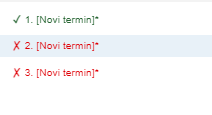
\includegraphics[scale=0.6]{dijagrami/test3.PNG}
	\centering
	\caption{Ispitni slučaj 3. rezultati}
	\label{fig:myChart}
\end{figure}

\begin{figure}[H]
	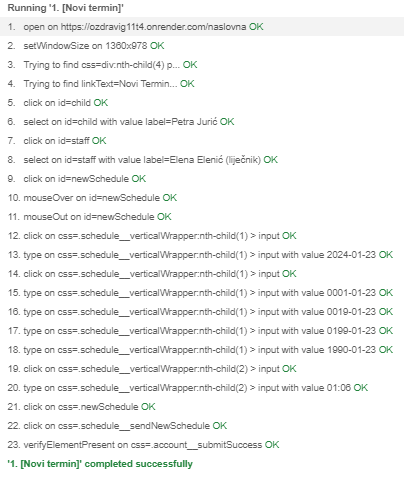
\includegraphics[scale=0.6]{dijagrami/test31.PNG}
	\centering
	\label{fig:myChart}
\end{figure}

\begin{figure}[H]
	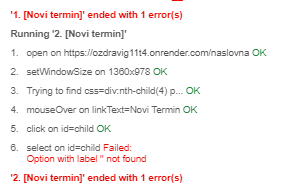
\includegraphics[scale=0.6]{dijagrami/test32.PNG}
	\centering
	\label{fig:myChart}
\end{figure}

\begin{figure}[H]
	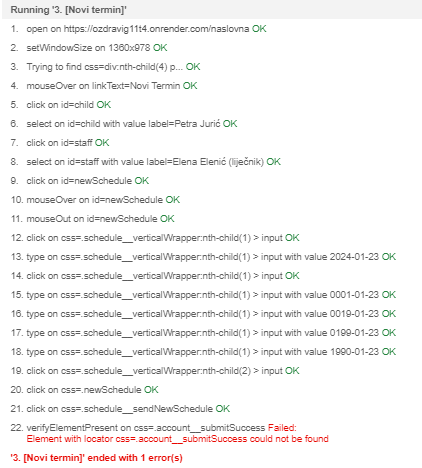
\includegraphics[scale=0.6]{dijagrami/test33.PNG}
	\centering
	\label{fig:myChart}
\end{figure}



\noindent	\textbf{Ispitni slučaj 4: Interakcija s sučeljem roditelja za slanje nalaza}
\\
\noindent \textbf{Ulaz:}
\begin{packed_enum}
	\item Otvaranje stranice s putanjom "/naslovna/noviTermin".
	\item Odabir dijeteta iz padajućeg izbornika.
	\item Odabir medicinskog osoblja iz padajućeg izbornika.
	\item Odabir opcije "Želim prenijeti nalaz"
	\item Prijenos datoteke
	\item Pritisak na akciju "Pošalji".
\end{packed_enum}

\noindent \textbf{Očekivani rezultat:}
\begin{packed_enum}
	\item Uspješna slanje i pohrana nalaza u sustav.
	\item Prikaz potvrdne poruke o uspješnom slanju.
\end{packed_enum}

\noindent \textbf{Redovni i rubni slučajevi:}
\begin{packed_enum}
	\item Korisnik je unio sve ispravne podatke.
	\item Korisnik nije odabrao dijete ili medicinsko osoblje iz padajućeg izbornika.
	\item Korisnik nije unio nalaz za prijenos.
\end{packed_enum}

\noindent \textbf{Rezultati:}
\begin{packed_enum}
	\item Korisnik je uspješno poslao zahtjev za novim terminom.
	\item Korisnik nije imao mogućnost daljnje ispune zahtjeva za terminom.
	\item Korisnik nije imao mogućnost pokretanja akcije "Pošalji".
\end{packed_enum}


\eject 
		
		
		\section{Dijagram razmještaja}
			
			\textbf{\textit{dio 2. revizije}}
			
			 \textit{Na poslužiteljskom računalu se nalaze web poslužitelj i poslužitelj baze podataka. Korisnici koriste web preglednik za pristup web aplikaciji. Sustav je baziran na arhitekturi ”klijent – poslužitelj”, a komunikacija između računala korisnika i poslužitelja odvija se preko HTTP veze.}
			
			\begin{figure}[H]
				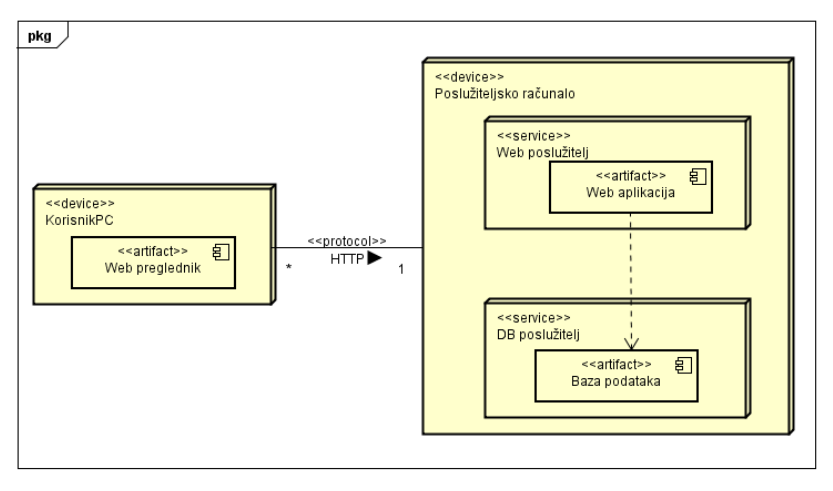
\includegraphics[width=15cm, height=12cm]{dijagrami/dijagram_razmjestaja.png}
				\caption{Dijagram razmještaja}
				\label{fig:classD}
			\end{figure}
			
			\eject 
		
		\section{Upute za puštanje u pogon}
		
			\textbf{\textit{dio 2. revizije}}\\
		
			 \textit{U ovom poglavlju potrebno je dati upute za puštanje u pogon (engl. deployment) ostvarene aplikacije. Na primjer, za web aplikacije, opisati postupak kojim se od izvornog kôda dolazi do potpuno postavljene baze podataka i poslužitelja koji odgovara na upite korisnika. Za mobilnu aplikaciju, postupak kojim se aplikacija izgradi, te postavi na neku od trgovina. Za stolnu (engl. desktop) aplikaciju, postupak kojim se aplikacija instalira na računalo. Ukoliko mobilne i stolne aplikacije komuniciraju s poslužiteljem i/ili bazom podataka, opisati i postupak njihovog postavljanja. Pri izradi uputa preporučuje se \textbf{naglasiti korake instalacije uporabom natuknica} te koristiti što je više moguće \textbf{slike ekrana} (engl. screenshots) kako bi upute bile jasne i jednostavne za slijediti.}
			
			
			 \textit{Dovršenu aplikaciju potrebno je pokrenuti na javno dostupnom poslužitelju. Studentima se preporuča korištenje neke od sljedećih besplatnih usluga: \href{https://aws.amazon.com/}{Amazon AWS}, \href{https://azure.microsoft.com/en-us/}{Microsoft Azure} ili \href{https://www.heroku.com/}{Heroku}. Mobilne aplikacije trebaju biti objavljene na F-Droid, Google Play ili Amazon App trgovini.}
			
			
			\eject 
